\documentclass[11pt, a4paper]{report}
%--------------Importación de paquetes (preámbulo)--------------%
\input{preambulo}
\usepackage[pdftex,
            pdfauthor={Joseph Jaramillo},
            pdftitle={Informe reporte sísmico},
            pdfsubject={UTN},
            pdfkeywords={Computer UNIVAC Evolutionary},
            pdfproducer={TeXLive},
            pdfcreator={pdflatex, or other tool},
            colorlinks=true,
            linkcolor=blue]{hyperref}


%---------------------------------------------------------------%
\graphicspath{ {../Figures/} }
\setlength{\parindent}{0em}
\topmargin=0.5cm
\usepackage[lmargin=2cm,rmargin=2cm,bottom=1cm]{geometry}
%%%%%% --- generando caja de pagina como background
\DefineNamedColor{named}{Cyan}{cmyk}{250,250,250,250}
\backgroundsetup{
scale=1,
angle=0,
color=Cyan,
opacity=1,
contents={
\begin{tikzpicture}[overlay,remember picture]
\draw [line width=1.5pt]
    ($ (current page.north west) + (1.0cm,-1.0cm) $) % izquierda, arriba
    rectangle
    ($ (current page.south east) + (-1.0cm,0.8 cm) $);  % derecha,abajo
\draw [line width=1.25pt]
    ($ (current page.north west) + (1.15cm,-1.15cm) $)
    rectangle
    ($ (current page.south east) + (-1.15cm,0.95cm) $); 
\end{tikzpicture}
}
}

%---------------------------------------------------------------%
\title{CENTRO DE MONITOREO SÍSMICO DEL CISMID-FIC-UNI \\
RED NACIONAL DE ACELERÓGRAFOS (REDACIS)\\
INFORME PRELIMINAR\\
}

%%  -------Encabezado -------%%%
\lhead{\vspace{-1cm} \begin{picture}(0,0) \put(0,0){
\includegraphics[width=18mm]{Logos/logo_uni}} \end{picture}}
\rhead{\vspace{-1cm} \begin{picture}(0,0) \put(-70,0){
\includegraphics[width=27mm]{Logos/logo_cismid}} \end{picture}}
\chead{\vspace{-0.5cm} UNIVERSIDAD NACIONAL DE INGENIERÍA\\
FACULTAD DE INGENIERÍA CIVIL\\
CENTRO PERUANO JAPONÉS DE INVESTIGACIONES\\
SÍSMICAS Y MITIGACIÓN DE DESASTRES\\
\vspace{-0.5cm} }


\renewcommand{\headrulewidth}{1pt}
\renewcommand{\headrule}{\hbox to\headwidth{\color{Cyan}\leaders\hrule height \headrulewidth\hfill}}
\renewcommand{\footrulewidth}{1pt}
\renewcommand{\footrule}{{\color{Cyan}\vskip-\footruleskip\vskip-\footrulewidth \hrule width\headwidth height\footrulewidth\vskip\footruleskip}}
%\futurelet\TMPfootrule\def\footrule{{\color{blue}\TMPfootrule}}
\setlength\headheight{40.0pt}
\addtolength{\textheight}{-100.0pt}
\cfoot{\scriptsize AV. TÚPAC AMARU N° 1150 – LIMA 25 – PERÚ – Apartado Postal 31-250 Lima 31\\
		Teléfono (511)482-0777, (511)482-0804, (511)482-0790   Fax: (511)481-0170 \\
		e-mail: director@uni.edu.pe   http://www.cismid.uni.edu.pe
		}

\pagestyle{fancy}

%%%%%
%-------------------CUERPO-------------------%
\begin{document}

\begin{pycode}
lugar = 'Lamas'
fecha = '20 de Noviembre del 2020'
hora = '01:38:24'
hora_UTC = '06:38:02'
referencia = '75 km sureste de Lagunas, Loreto'
institucion = 'IGP'
latitud = '-9.95'
longitud = '-78.96'
profundidad = '46'
magnitud = '5.7'
nstations = 3
\end{pycode}

\begin{center}
\centering 
\textbf{CENTRO DE MONITOREO SÍSMICO DEL CISMID-FIC-UNI \\
RED DE MONITOREO DE EDIFICACIONES}
\vspace{0.3cm}

\textbf{INFORME PRELIMINAR}
\vspace{0.3cm}

\textbf{Acelerogramas del Sismo de \py{lugar} del \py{fecha}}
\vspace{0.25cm}
\end{center}

El \py{fecha} a las \py{hora} (hora local), ocurrió un sismo con epicentro a \py{referencia} (Fuente: \py{institucion}). Las características sísmicas del evento 
se resumen en la Tabla (\ref{tab:tab01}) y la ubicación del epicentro, así como de las estaciones 
acelerográficas más cercanas, se muestra en la Figura (\ref{tab:tab01}). \\

\begin{figure}[H]
    \begin{multicols}{2}
        \begin{minipage}[c]{7.5cm}
            \centering
            \renewcommand{\arraystretch}{1.8}
            \captionof{table}{Datos sísmicos (Fuente: \py{institucion})} \label{tab:tab01}
            \begin{tabulary}{7.0cm}{|l|C|}
                
            \hline
            Hora local (UTC-5): & \py{hora} \\ \hline
            Hora UTC 0: & \py{hora_UTC} \\ \hline
            Latitud ($^{\circ}$): & \py{latitud} \\ \hline
            Longitud ($^{\circ}$): & \py{longitud} \\ \hline
            Profundidad (km): & \py{profundidad} \\ \hline
            Magnitud (ML): & \py{magnitud} \\ \hline
            Lugar de referencia: & \py{referencia}. \\ 
            \hline
            \end{tabulary}
        \end{minipage}
    
        \hspace{0.5cm}
    
        \begin{minipage}[c]{8.2cm}
            \centering %%\captionsetup{format = hang, width=8cm}
            \setlength\fboxsep{0pt}
            \setlength\fboxrule{0.3pt}
            \captionof{figure}{Epicentro y estaciones cercanas.}  \label{fig:fig01}
            % \begin{figure}
                \fbox{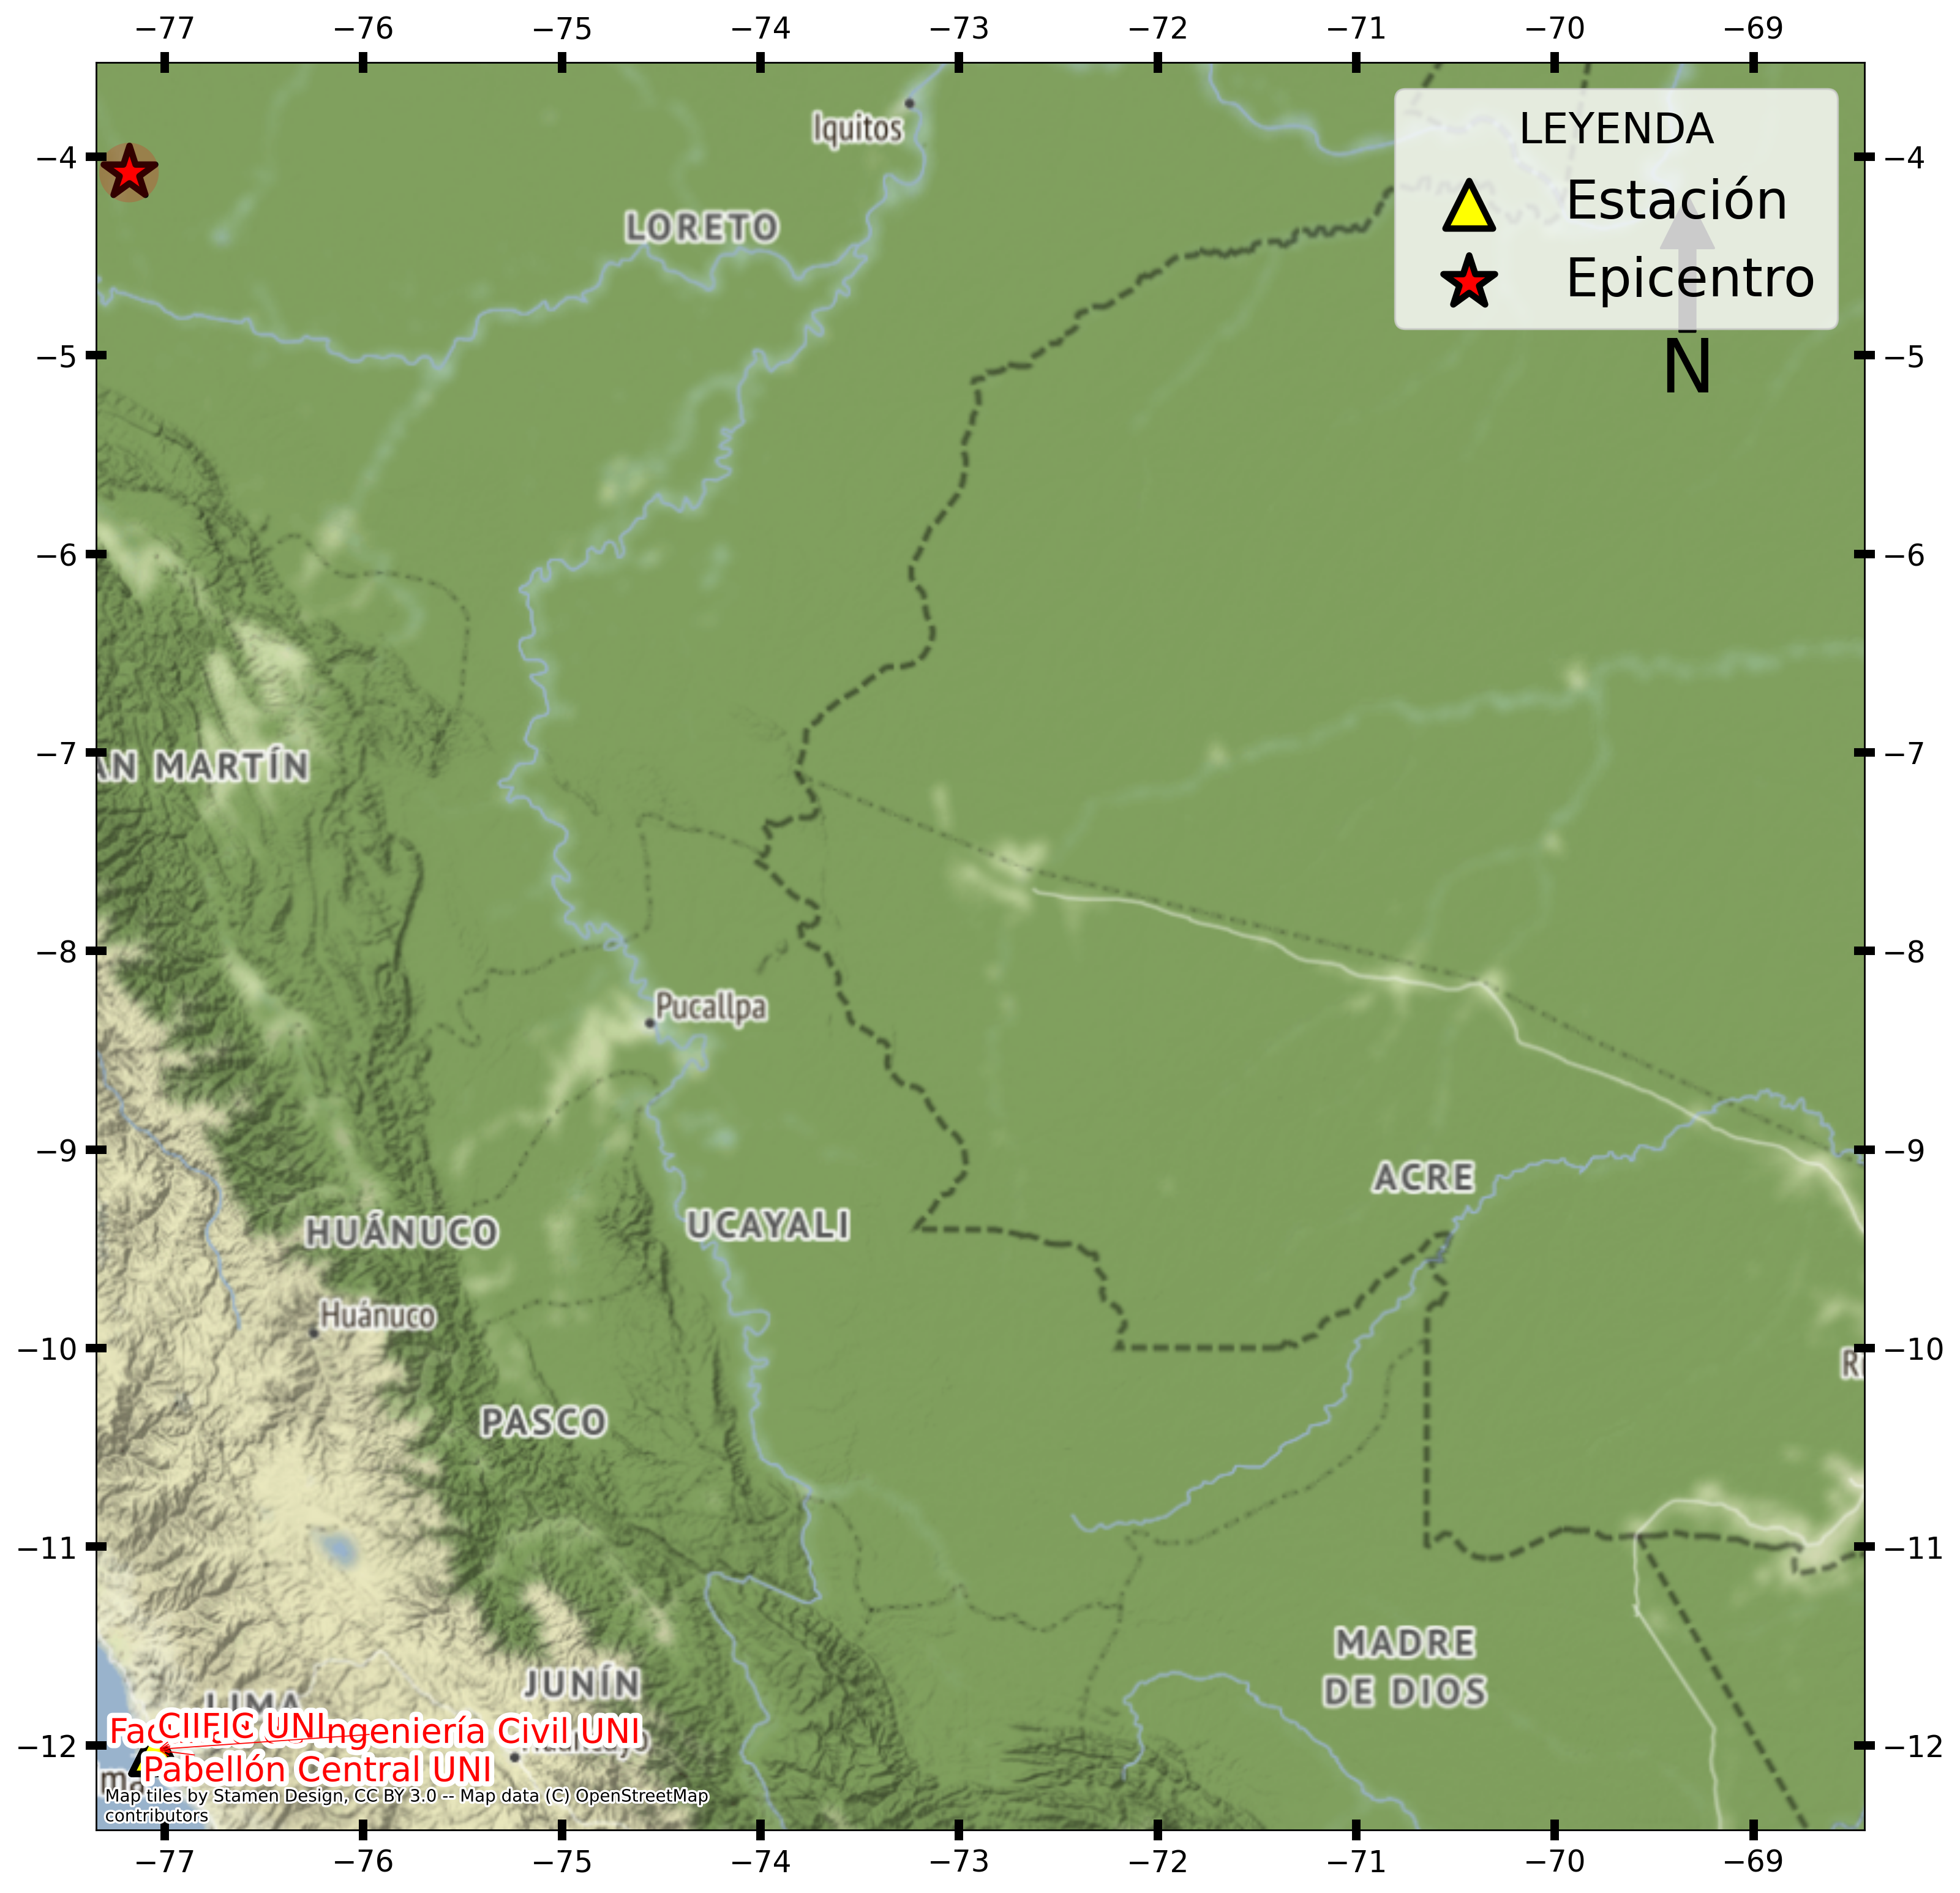
\includegraphics[trim={1mm 0.5mm 1mm 0.5mm},clip,width=1.0\textwidth]{Mapa01.png}}
            % \end{figure}
        \end{minipage}
    \end{multicols} 
\end{figure}

\vspace{1cm}

\noindent
En este reporte, la Red de Monitoreo de Edificaciones del CISMID-FIC-UNI (REMOED) presenta de manera
preliminar, los registros sísmicos obtenidos de este evento correspondiente a \py{nstations} estaciones 
acelerográficas ubicadas en la ciudad de Lima, cuyos valores de aceleración máxima, para cada 
componente, y localizaciónes se muestran en la Tabla (\ref{tab:tab02}) y Figura (\ref{fig:fig02}) respectivamente.\\

\begin{pycode}
import pandas as pd

PGA_max = 3.55
direccion = 'NS'
stationmax = 'FIC-UNI'
stationmaxubic = 'FIC-UNI, Rímac, Lima'

cap_fig2 = "Aceleraciones máximas registrados en las estaciones acelerográficas ubicadas en la ciudad de Lima correspondientes al sismo de {0} del {1} a las {2} (hora local)".format(lugar, fecha, hora)

station = pd.DataFrame({'Latitude': [-12.1740, -12.0976, -12.0605], 
                        'Longitude': [-77.0191, -77.0172, -76.9759], 
                        'Name': ['CIIFIC', 'FIC-UNI', 'CISMID'], 
                        'Location':['CIIFIC-FIC-UNI, Rímac, Lima', 'FIC-UNI, Rímac, Lima', 'CISMID-FIC-UNI, Rímac, Lima'],
                        'PGA':[[3.54, 3.55, 1.52], [-1.04, -1.00, -0.76], [-1.19, 1.43, -1.07]]
                        })

\end{pycode}

\newpage
\noindent
El máximo valor de PGA registrado en estas estaciones es de \py{PGA_max} cm/s2 en la dirección \py{direccion} 
correspondiente a la estación \py{stationmax} (\py{stationmaxubic}).
Finalmente, en el Anexo adjunto se presentan las gráficas de los acelerogramas obtenidos 
en las trece estaciones (direcciones EW, NS y vertical).

\begin{pycode}

print(r"\renewcommand{\arraystretch}{1.2}")
print(r"\begin{longtable}{|c|c|c|c|}")
print(r"\caption{%s}\label{tab:tab02}\\"%(cap_fig2))
print(r"\hline")
print(r"\textbf{Código} & \textbf{Orientación} & \textbf{Ubicación (Provincia, Departamento)} & \textbf{\begin{tabular}[c]{@{}c@{}}PGA\\ (cm/s2)\end{tabular}} \\ \hline")
# print(r"\hline")
print(r"\endfirsthead")
# print(r"\hline")
# print(r"\textbf{Código} & \textbf{Orientación} & \textbf{Ubicación (Provincia, Departamento)} & \textbf{\begin{tabular}[c]{@{}c@{}}PGA\\ (cm/s2)\end{tabular}} \\ \hline")
# print(r"\hline")
print(r"\endhead")
print(r"\endfoot")
print(r"\endlastfoot")

for i in range(len(station)):
    print(r"\multirow{3}{*}{%s}"%(station["Name"][i]),r" & EW & \multirow{3}{*}{\begin{tabulary}{8cm}{@{}C@{}} %s\end{tabulary}}"%(station["Location"][i]),r" & %.2f \\ \cline{2-2} \cline{4-4}"%(station["PGA"][i][0]))
    print(r" & NS &  & %.2f \\ \cline{2-2} \cline{4-4}"%(station["PGA"][i][1]))
    print(r" & UD &  & %.2f \\ \hline"%(station["PGA"][i][2]))
    if (i+1) == 9 or (i-8) % 11 == 0:
        print(r"\pagebreak")
print(r"\end{longtable}")

print(r"\newpage")

\end{pycode}


\begin{figure}[!h]
    \centering
            \caption{Mapa de ubicación de las estaciones acelerográficas en la ciudad de Lima}
            \label{fig:fig02}
            \setlength\fboxsep{0pt}
            \setlength\fboxrule{0.3pt}
            \fbox{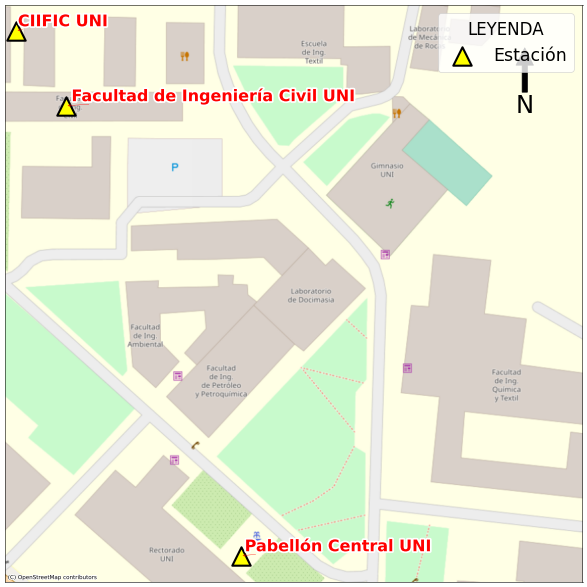
\includegraphics[trim={1mm 1mm 1mm 1mm},clip,width=\textwidth]{Mapa02.png}}
    
    \end{figure}
    
\end{document}

